\chapter{CSP Models for Puzzler Games}
\label{cha:design}
Generally, this chapter mainly discusses 3 parts: the analysis of the rotation matrices, the model of the 2D game (IQ twist) and the two playing modes of models for the 3D game (ZIG ZAG puzzler). The analysis of rotation matrices makes it clear how we create the constraints for each game. The 2D game and 3D game parts introduce their models separately.
\section{Rotation Matrix}
"Rotation is the action of moving or causing to move in a circle round an axis or centre" \cite{r14}. For a vector, the length of the vector will be reserved after rotation. Meanwhile, the process can be represented by matrix operation such as 
\begin{equation}
Y=M.X,
\end{equation}
where $X$ is the input vector, $M$ is the rotation matrix and $Y$ is the output vector \cite{r15}. Therefore, the rotation matrices can be used to mathematically define rotations that can describe the placements for the pieces of the two games. The 2D rotation matrix is corresponding to IQ twist and the 3D rotation matrix is corresponding to ZIG ZAG puzzler. In our case, only counter-clockwise rotations of 90, 180 and 270 degrees for both 2D (the xy-plane) and 3D (the xy-plane, the yz-plane and the xz-plane) will be considered.
\subsection{2D Rotation Matrix}
Tobias and Krantz \cite{r9} mention that 2D rotation can be described by a matrix
\begin{equation}
R(\theta)=\begin{bmatrix}
\cos\theta & -\sin\theta\\
\sin\theta & \cos\theta\\
\end{bmatrix}.
\end{equation}
If the initial position is (x,y), we can get the position after the rotation by
\begin{equation}
\begin{bmatrix}
x'\\
y'\\
\end{bmatrix}
=\begin{bmatrix}
\cos\theta & -\sin\theta\\
\sin\theta & \cos\theta\\
\end{bmatrix}
\begin{bmatrix}
x\\
y\\
\end{bmatrix},
\end{equation}
which implies that 
\begin{equation}
\begin{aligned}
&x'=x\cos\theta-y\sin\theta,\\
&y'=x\sin\theta+y\cos\theta.
\end{aligned}
\end{equation}
Therefore, if we assign 0, 90, 180 and 270 degrees to the $\theta$, we get 4 situations:
\begin{itemize}
  \item $x'=x\cos0^{\circ} - y\sin0^{\circ}\hspace{20pt},y'=x\sin0^{\circ} + y\cos0^{\circ}\hspace{24pt}\implies x'=x\hspace{10pt}, y'=y$
  \item $x'=x\cos90^{\circ} - y\sin90^{\circ}\hspace{10pt},y'=x\sin90^{\circ} + y\cos90^{\circ}\hspace{12pt}\implies x'=-y, y'=x$
  \item $x'=x\cos180^{\circ} - y\sin180^{\circ}, y'=x\sin180^{\circ} + y\cos180^{\circ} \implies x'=-x, y'=-y$
  \item $x'=x\cos270^{\circ} - y\sin270^{\circ}, y'=x\sin270^{\circ} + y\cos270^{\circ} \implies x'=y\hspace{10pt},y'=-x$
  \label{rotation4}
\end{itemize}
In IQ twist, there exists mirroring operation, if a point flip over around the y-axis, we get  (-x,y) from (x,y). Similarly, all the 4 situations flip over around the y-axis. we get 4 more situations: 
\begin{itemize}
  \item  $x'=x\hspace{10pt}, y'=y\hspace{10pt}$    flip over around the y-axis $\implies x''=-x\hspace{8pt},y''=y$
  \item  $x'=-y, y'=x\hspace{10pt}$                flip over around the y-axis $\implies x''=y,y''=x$
  \item  $x'=-x, y'=-y$               flip over around the y-axis $\implies x''=x, y''=-y$
  \item  $x'=y\hspace{10pt},y'=-x$    flip over around the y-axis $\implies x''=-y\hspace{8pt}, y''=-x$
  \label{mirrorrotate4}
\end{itemize}
Therefore, there should be total 8 situations for each unit of pieces. However, there might be some special situations like x=1, y=1. In such a case, according to the 8 formulas, there are only 4 situations because 4 of them are repeated.
\subsection{3D Rotation Matrix}
There are two forms to represent 3D rotations \cite{r9}. One is 3 separated matrices,
\begin{equation}
\begin{aligned}
R_{x}(\theta)=\begin{bmatrix}
1&          0&          0\\
0&\cos\theta & -\sin\theta\\
0&\sin\theta & \cos\theta\\
\end{bmatrix}
R_{y}(\theta)=\begin{bmatrix}
  \cos\theta&          0&\sin\theta\\
           0&          1& 0\\
-\sin\theta &          0&\cos\theta\\
\end{bmatrix},
R_{z}(\theta)=\begin{bmatrix}
\cos\theta&-\sin\theta&0\\
\sin\theta& \cos\theta&0\\
         0&          0&1\\
\end{bmatrix}
\end{aligned}
\end{equation}
,where $R_{x}(\theta)$ is corresponding to the yz-plane, $R_{y}(\theta)$ is corresponding to the xz-plane and $R_{z}(\theta)$ is corresponding to the xy-plane. The other is the combination of the 3 matrices in (3.5), 
\begin{equation}
\begin{aligned}
&R=R_{z}(\alpha)R_{y}(\beta)R_{x}(\gamma)=\\
&\begin{bmatrix}
\cos\alpha\cos\beta&\cos\alpha\sin\beta\sin\gamma-\sin\alpha\cos\gamma&\cos\alpha\sin\beta\cos\gamma+\sin\alpha\sin\gamma\\
\sin\alpha\cos\beta&\sin\alpha\sin\beta\sin\gamma+\cos\alpha\cos\gamma&\sin\alpha\sin\beta\cos\gamma-\cos\alpha\sin\gamma\\
         -\sin\beta&                               \cos\beta\sin\gamma&\cos\beta\cos\gamma\\
\end{bmatrix}.
\end{aligned}
\end{equation}
compared with the 2D rotation matrix, the 3D rotation matrices will consider more planes. But there are still some similarities. For example,
\begin{equation}
\begin{aligned}
&x'=x\cos\theta-y\sin\theta,\\ 
&y'=x\sin\theta+y\cos\theta,\\
&z'=z
\end{aligned}
\end{equation}
can be derived from
\begin{equation}
\begin{bmatrix}
x'\\
y'\\
z'\\
\end{bmatrix}
=R_{z}(\theta)
\begin{bmatrix}
x\\
y\\
z\\
\end{bmatrix}
\end{equation}
The forms of the x' and the y' in (3.8) are the same with (3.4), the only difference is that this formula takes Z into account. In addition, mirroring operation in 2D can be seen as a special case of 3D rotation. It is the same with rotating around the xz-plane 180 degrees Because 
\begin{equation}
\begin{aligned}
&x'=-x,\\
&y'=-y,\\
&z'=-z
\end{aligned}
\end{equation}
can be derived from 
\begin{equation}
\begin{bmatrix}
x'\\
y'\\
z'\\
\end{bmatrix}
=R_{y}(180^{\circ})
\begin{bmatrix}
x\\
y\\
z\\
\end{bmatrix},
\end{equation}
and $z$ will be ignored in 2D rotation.\\
In our case, we only consider 90, 180 and 270 degrees rotations for each plane. If we separately consider each plane. There should be 4 situations for each plane. For example, $\theta=0^{\circ}, 90^{\circ}, 180^{\circ}, 270^{\circ}$ in (3.8) is corresponding to the xy-plane. Similarly, the yz-plane and xz-plane can get 4 situations each. Then we combine all of them, there should be 64 situations ($4\times 4 \times 4$). However, there are only 24 situations because of the "singularity" of Euler angles set, the geometric singularity will appear when $\beta=\pm90^{\circ}$ 
as well as $\beta=0^{\circ}$ or $180^{\circ}$ \cite{r17}. Now we consider $\beta=\pm90^{\circ}$. If $\beta=90^{\circ}$, we get 
\begin{equation}
R_{\beta=90}=R_{z}(\alpha)R_{y}(90^{\circ})R_{x}(\gamma)=
\begin{bmatrix}
0&-\sin(\alpha-\gamma)&\cos(\alpha-\gamma)\\
0&\cos(\alpha-\gamma)&\sin(\alpha-\gamma)\\
         -1&                              0&0\\
\end{bmatrix}.
\end{equation}
And when $\beta=-90^{\circ}$, it can be seen as $\beta=270^{\circ}$ because of the periodicity, we can get 
\begin{equation}
R_{\beta=270}=R_{z}(\alpha)R_{y}(270^{\circ})R_{x}(\gamma)=
\begin{bmatrix}
0&-\sin(\alpha+\gamma)&-\cos(\alpha+\gamma)\\
0&\cos(\alpha+\gamma)&-\sin(\alpha+\gamma)\\
1&                               0&0
\end{bmatrix}.
\end{equation}
Based on the formula
\begin{equation}
\begin{bmatrix}
x'\\
y'\\
z'\\
\end{bmatrix}
=R
\begin{bmatrix}
x\\
y\\
z\\
\end{bmatrix},
\end{equation}
for $\beta=90^{\circ}$,
\begin{equation}
\begin{aligned}
&x'=-y\sin(\alpha-\gamma)-z\cos(\alpha-\gamma), \\
&y'=y\cos(\alpha-\gamma)+z\sin(\alpha-\gamma), \\
&z'=-x. 
\end{aligned}
\end{equation}
and for $\beta=270^{\circ}$, 
\begin{equation}
\begin{aligned}
&x'=-y\sin(\alpha+\gamma)-z\cos(\alpha+\gamma), \\
&y'=y\cos(\alpha+\gamma)-z\sin(\alpha+\gamma), \\
&z'=x.
\end{aligned}
\end{equation}
Because in our case, the domains of both $\alpha$ and $\gamma$ are $0^{\circ}$, $90^{\circ}$, $180^{\circ}$, $270^{\circ}$ and the period of the trigonometric function is $360^{\circ}$. For (3.14), the 4 situations are $\alpha-\gamma$=$0^{\circ}$ or $90^{\circ}$ or $180^{\circ}$ or $270^{\circ}$. For (3.15), the 4 situations are $\alpha+\gamma$=$0^{\circ}$ or $90^{\circ}$ or $180^{\circ}$ or $270^{\circ}$. Therefore, these 2 groups of formulas represent that there are only 4 situations for each of them. In other words, the separated $\alpha$ and $\gamma$ are meaningless. What we should consider is $\alpha-\gamma$ for (3.14) and $\alpha+\gamma$ for (3.15).\\ 
Then, we consider  $\beta=0^{\circ}$ and $\beta=180^{\circ}$. Based on (3.6), when $\beta=0^{\circ}$, we get
\begin{equation}
R=R_{z}(\alpha)R_{y}(0^{\circ})R_{x}(\gamma)=
\begin{bmatrix}
\cos\alpha&-\sin\alpha\cos\gamma&\sin\alpha\sin\gamma\\
\sin\alpha&\cos\alpha\cos\gamma&-\cos\alpha\sin\gamma\\
0&          \sin\gamma&\cos\gamma\\
\end{bmatrix}.
\end{equation}
When $\beta=180^{\circ}$, we get
\begin{equation}
R=R_{z}(\alpha)R_{y}(180^{\circ})R_{x}(\gamma)=
\begin{bmatrix}
-\cos\alpha&-\sin\alpha\cos\gamma&\sin\alpha\sin\gamma\\
-\sin\alpha&\cos\alpha\cos\gamma&-\cos\alpha\sin\gamma\\
0&                               -\sin\gamma&-\cos\gamma\\
\end{bmatrix}.
\end{equation}
In (3.17), we assign $\alpha=\alpha+180^{\circ}$ and $\gamma=\gamma+180^{\circ}$, then it change to
\begin{equation}
\begin{aligned}
&R=R_{z}(\alpha+180^{\circ})R_{y}(180^{\circ})R_{x}(\gamma+180^{\circ})=\\
&\begin{bmatrix}
-\cos(\alpha+180^{\circ})&-\sin(\alpha+180^{\circ})\cos(\gamma+180^{\circ})&\sin(\alpha+180^{\circ})\sin(\gamma+180^{\circ})\\
-\sin(\alpha+180^{\circ})&\cos(\alpha+180^{\circ})\cos(\gamma+180^{\circ})&-\cos(\alpha+180^{\circ})\sin(\gamma+180^{\circ})\\
0&                               -\sin(\gamma+180^{\circ})&-\cos(\gamma+180^{\circ})
\end{bmatrix}\\
&=\begin{bmatrix}
\cos(\alpha)&-\sin(\alpha)\cos(\gamma)&\sin(\alpha)\sin(\gamma)\\
\sin(\alpha)&\cos(\alpha)\cos(\gamma)&-\cos(\alpha)\sin(\gamma)\\
0&                               \sin(\gamma)&\cos(\gamma)\\
\end{bmatrix}.
\end{aligned}
\end{equation}
Therefore, based on (3.16) and (3.18),
\begin{equation}
R_{z}(\alpha)R_{y}(0^{\circ})R_{x}(\gamma)=R_{z}(\alpha+180^{\circ})R_{y}(180^{\circ})R_{x}(\gamma+180^{\circ})
\end{equation}, 
which means that when $\beta=0^{\circ}$, regardless of the number of degrees of $\alpha$ and the number of degrees of $\gamma$, there are always corresponding $\alpha+180^{\circ}$, $\gamma+180^{\circ}$ when $\beta=180^{\circ}$. Even though the number of degrees of $\alpha+180^{\circ}$ or $\gamma+180^{\circ}$ may be more than $360^{\circ}$, it can always find a corresponding from $0^{\circ}$ to $360^{\circ}$ according to the periodicity of trigonometric function. For example, \begin{equation}
\begin{aligned}
&\circled{1}R_{z}(270^{\circ})Ry(0^{\circ})R_{x}(270^{\circ}) = R_{z}(450^{\circ})R_{y}(180^{\circ})R_{x}(450^{\circ})\\ 
&\circled{2}R_{z}(450^{\circ})Ry(180^{\circ})R_{x}(450^{\circ}) = R_{z}(90^{\circ})R_{y}(180^{\circ})R_{x}(90^{\circ})\\
&\circled{1},\circled{2}\implies R_{z}(270^{\circ})Ry(0^{\circ})R_{x}(270^{\circ})   = R_{z}(90^{\circ})R_{y}(180^{\circ})R_{x}(90^{\circ}).
\end{aligned}
\end{equation}
Hence, all combinations among $\beta=0^{\circ}$, $\theta=0^{\circ}$ or $90^{\circ}$ or $180^{\circ}$ or $270^{\circ}$ and $\gamma=0^{\circ}$ or $90^{\circ}$ or $180^{\circ}$ or $270^{\circ}$ can be obtained from one combination among $\beta=180^{\circ}$, $\theta=0^{\circ}$ or $90^{\circ}$ or $180^{\circ}$ or $270^{\circ}$ and $\gamma=0^{\circ}$ or $90^{\circ}$ or $180^{\circ}$ or $270^{\circ}$. So we only need to consider the all situations when $\beta=0^{\circ}$ because the all situations in $\beta=180^{\circ}$ are duplicates. There should be a total of 16 situations (4$\times$4). Finally, consider the all situations in $\beta=90^{\circ}$,$\beta=270^{\circ}$,$\beta=^{\circ}0$ and $\beta=180^{\circ}$. There should be a total of 4+4+16=24 situations.
\section{IQ Twist}
In this part, the design of CSP model for IQ twist will be discussed. 
\subsection{Variables}
Above all, the initial state of each piece is defined in Figure 3.1. For this method, there are some rules. Firstly, all the variables are corresponding to the initial states. Such as the yellow2, Figure 3.2 shows that the $V_{y21}$ is used to represent the left and bottom unit. For other variables, we name them as $V_{y22}$, $V_{y23}$, $V_{y24}$ and $V_{y25}$, which follows the order from left to right and bottom-up. In addition, there are 7 pegs. Therefore, the variables can be represented as \VUnits and \VPegs.
\begin{figure}[htbp]
\begin{subfigure}[b]{.24\textwidth}
\centering

\includegraphics[width=0.75\textwidth]{figs/yellow1.jpg}
\caption{Initial state of yellow1}
  \label{fig:2Dyellow1}
\end{subfigure}
\begin{subfigure}[b]{.24\textwidth}
\centering
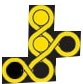
\includegraphics[width=0.75\textwidth]{figs/yellow2.jpg}
\caption{Initial state of yellow2}
  \label{fig:2Dyellow2}
\end{subfigure}
\begin{subfigure}[b]{.24\textwidth}
\centering
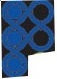
\includegraphics[width =0.5\textwidth]{figs/blue1.jpg}
\caption{Initial state of blue1}
  \label{fig:2Dblue1}
\end{subfigure}
\begin{subfigure}[b]{.24\textwidth}
\centering

\includegraphics[width=\textwidth]{figs/blue2.jpg}
\caption{Initial state of blue2}
  \label{fig:2Dblue2}
\end{subfigure}
\begin{subfigure}[b]{.24\textwidth}
\centering

\includegraphics[width=0.75\textwidth]{figs/green1.jpg}
\caption{Initial state of green1}
  \label{fig:2Dgreen1}
\end{subfigure}
\begin{subfigure}[b]{.24\textwidth}
\centering

\includegraphics[width =0.5\textwidth]{figs/green2.jpg}
\caption{Initial state of green2}
  \label{fig:2Dgreen2}
\end{subfigure}
\begin{subfigure}[b]{.24\textwidth}
\centering

\includegraphics[width =\textwidth]{figs/red1.jpg}
\caption{Initial state of red1}
  \label{fig:2Dred1}
\end{subfigure}
\begin{subfigure}[b]{.24\textwidth}
\centering

\includegraphics[width=0.75\textwidth]{figs/red2.jpg}
\caption{Initial state of red2}
  \label{fig:2Dred2}
\end{subfigure}
\caption{Initial state of each piece}
  \label{fig:allinit}
\end{figure}
\begin{figure}[htbp]
    \centering
    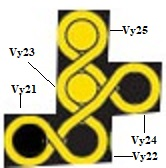
\includegraphics[width=0.3\textwidth]{figs/example.jpg}
    \caption{Name rules for yellow2}
    \label{fig:namerules}
\end{figure}
\begin{align*}
\VUnits=\{&V_{y11},V_{y12},V_{y13},\\&V_{y21},V_{y22},V_{y23},V_{y24},V_{y25},\\&V_{b11},V_{b12},V_{b13},V_{b14},
V_{b15},\\&V_{b21},V_{b22},V_{b23},V_{b24},\\&V_{g11},V_{g12},V_{g13},V_{g14},\\&V_{g21},V_{g22},V_{g23},\\&V_{r11},
V_{r12},V_{r13},V_{r14},\\&V_{r21},V_{r22},V_{r23},V_{r24}\}\\
\\\VPegs = \{&V_{py1}, V_{py2}, V_{pb1}, V_{pb2}, V_{pg1}, V_{pg2}, V_{pr}\}\\
\\V = &\VUnits \cup \VPegs.
\end{align*}
\subsection{Domains}
For the board, Figure 3.3 shows that the 2D coordinate system is used to represent the positions. In our model, the left and bottom position as (0,0) and the right and top as (8,4). So, all placements will be between them. The pegs are special, they can be put in any places on the board or not on the board.
\begin{figure}[htbp]
\centering
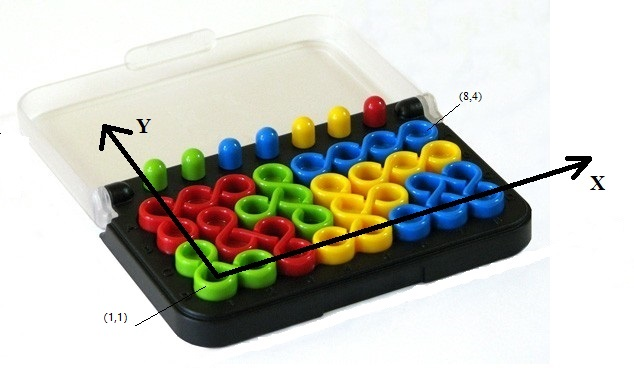
\includegraphics[width=0.8\textwidth]{figs/IQtwistboard.jpg}
\caption{The coordinate system for IQ twist}
    \label{fig:coordinate}
\end{figure}
\begin{align*}
&For \hspace{1ex} all \hspace{1ex} v \in \VUnits \hspace{1ex},\hspace{1ex} D(v)=\{(i,j) \in \mathbb{Z} \times \mathbb{Z}	\mid  0<i \leq 8 \hspace{1ex} , \hspace{1ex} 0<j \leq 4\}\\
\\
&For \hspace{1ex} all \hspace{1ex} v \in \VPegs \hspace{1ex},\hspace{1ex} D(v)=\{(0,0)\} \hspace{1ex} \cup \hspace{1ex}\{(i,j) \in \mathbb{Z} \times \mathbb{Z}\mid  0<i \leq 8 \hspace{1ex} , \hspace{1ex} 0<j \leq 4\}
\end{align*}
\subsection{Constrains}
Firstly, there should be no 2 different unit variables contain the same value. Similarly, there should be no 2 different reg variables contain the same value except both of them are not on the board. In Figure 3.4 , the unit which is corresponding to the first variable (here it is $V_{y21}$) will be considered as a point $(x,y)$. Therefore, the $V_{y21}$, $V_{y22}$, $V_{y23}$, $V_{y24}$ and $V_{y25}$ are respectively represented as $(x,y)$, $(x+1,y)$, $(x+1,x+1)$, $(x+2,y+1)$ and $(x+1,y+2)$, which indicates that all other variables can be connected with the first variables. In addition, all other placements can get from the initial state of the piece by rotations. According to 3.1.1, there are 8 rotation situations. Figure 3.5 points out all placements for yellow2. Furthermore, for the pegs, unless they are not on the board, there must be a hollow unit of pieces which contains the same color with the pegs to match them.
\begin{figure}[htbp]
\centering
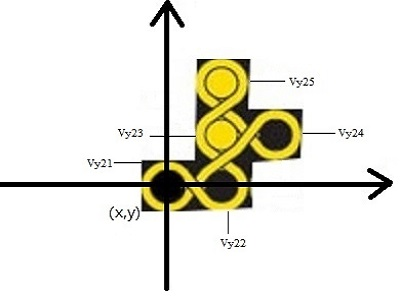
\includegraphics[width=0.5\textwidth]{figs/explanation2D.jpg}
\caption{The explanation of 2D rotation}
    \label{fig:explanation2D}
\end{figure}
\begin{figure}
\centering
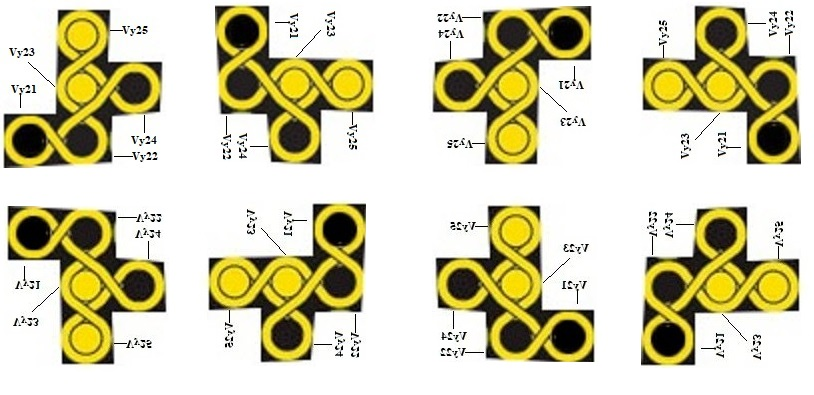
\includegraphics[width =\textwidth]{figs/domainexplain.jpg}
    \caption{Example of 8 situations}
    \label{fig:Exampleof8}
\end{figure} 
\\\circled{1} 
For each pair of variables $V_{m}$ and $V_{n}$, $V_{m} \in \VUnits$, $V_{n} \in \VUnits$,$V_{m} \neq V_{n}$,
\begin{center}
$\Constraints{m}{n}=\{((x_{1},y_{1}),(x_{2},y_{2}))\in \Domain{m} \times \Domain{n}\mid x_{1} \neq x_{2}   \hspace{1ex} or \hspace{1ex}  y_{1} \neq y_{2}\}$
\end{center}
\circled{2} 
For each pair of variables $V_{m}$ and $V_{n}$, $V_{m} \in \VPegs$, $V_{n} \in \VPegs$, $V_{m} \neq V_{n}$,
\begin{align*}
\Constraints{m}{n}=&\{((0,0),(0,0))\}\cup \\ 
&\{((x_{1},y_{1}),(x_{2},y_{2}))\in \Domain{m}\times \Domain{n}\mid x_{1} \neq x_{2}   \hspace{1ex} or \hspace{1ex}  y_{1} \neq y_{2}\}
\end{align*}
\\\circled{3} piece Yellow1
\begin{align*}
\Con{y11}{y12}{y13}=\{&((x_{1},y_{1}),(x_{2},y_{2}),(x_{3},y_{3}))\in \Domain{y11}\times \Domain{y12}\times\Domain{y13}\mid\\
&(x_{2} = x_{1} + 1,\hspace{1ex}y_{2} = y_{1},\hspace{1ex}x_{3} = x_{1} + 2, \hspace{1ex}y_{3} = y_{1})\hspace{1ex} or\\
&(x_{2} = x_{1},\hspace{1ex}y_{2} = y_{1}+1,\hspace{1ex}x_{3} = x_{1}, \hspace{1ex}y_{3} = y_{1}+2)\hspace{1ex} or\\
&(x_{2} = x_{1}-1,\hspace{1ex}y_{2} = y_{1},\hspace{1ex}x_{3} = x_{1}-2,\hspace{1ex} y_{3} = y_{1})\hspace{1ex} or\\
&(x_{2} = x_{1},\hspace{1ex}y_{2} = y_{1}-1,\hspace{1ex}x_{3} = x_{1}, \hspace{1ex}y_{3} = y_{1}-2)\hspace{3ex} \}
\end{align*} 
\\\circled{4} piece Yellow2
\begin{align*}
\Cons{y21}{y22}{y23}{y24}{y25}=\{&((x_{1},y_{1}),(x_{2},y_{2}),(x_{3},y_{3}),(x_{4},y_{4}),(x_{5},y_{5}))\in \\
&\Domain {y21} \times \Domain{y22}\times \Domain{y23}\times \Domain{y24}\times \Domain{y25} \mid\\
&(x_{2} = x_{1} + 1,\hspace{1ex}y_{2} = y_{1},\hspace{1ex}x_{3} = x_{1}+1,\hspace{1ex}y_{3} = y_{1}+1,
\\&x_{4} = x_{1}+2,\hspace{1ex}y_{4} = y_{1}+1,\hspace{1ex}x_{5} = x_{1}+1,\hspace{1ex}y_{5} = y_{1}+2)\hspace{1ex} or \\
&(x_{2} = x_{1} ,\hspace{1ex}y_{2} = y_{1}+1,\hspace{1ex}x_{3} = x_{1}-1,\hspace{1ex}y_{3} = y_{1}+1,
\\&x_{4} = x_{1}-1,\hspace{1ex}y_{4} = y_{1}+2,\hspace{1ex}x_{5} = x_{1}-2,\hspace{1ex}y_{5} = y_{1}+1)\hspace{1ex} or \\
&(x_{2} = x_{1}-1 ,\hspace{1ex}y_{2} = y_{1},\hspace{1ex}x_{3} = x_{1}-1,\hspace{1ex}y_{3} = y_{1}-1,
\\&x_{4} = x_{1}-2,\hspace{1ex}y_{4} = y_{1}-1,\hspace{1ex}x_{5} = x_{1}-1,\hspace{1ex}y_{5} = y_{1}-2)\hspace{1ex} or \\
&(x_{2} = x_{1} ,\hspace{1ex}y_{2} = y_{1}-1,\hspace{1ex}x_{3} = x_{1}+1,\hspace{1ex}y_{3} = y_{1}-1,
\\&x_{4} = x_{1}+1,\hspace{1ex}y_{4} = y_{1}-2,\hspace{1ex}x_{5} = x_{1}+2,\hspace{1ex}y_{5} = y_{1}-1)\hspace{1ex} or \\
&(x_{2} = x_{1}-1 ,\hspace{1ex}y_{2} = y_{1},\hspace{1ex}x_{3} = x_{1}-1,\hspace{1ex}y_{3} = y_{1}+1,
\\&x_{4} = x_{1}-2,\hspace{1ex}y_{4} = y_{1}+1,\hspace{1ex}x_{5} = x_{1}-1,\hspace{1ex}y_{5} = y_{1}+2)\hspace{1ex} or \\
&(x_{2} = x_{1} ,\hspace{1ex}y_{2} = y_{1}-1,\hspace{1ex}x_{3} = x_{1}-1,\hspace{1ex}y_{3} = y_{1}-1,
\\&x_{4} = x_{1}-1,\hspace{1ex}y_{4} = y_{1}-2,\hspace{1ex}x_{5} = x_{1}-2,\hspace{1ex}y_{5} = y_{1}-1)\hspace{1ex} or \\
&(x_{2} = x_{1}+1 ,\hspace{1ex}y_{2} = y_{1},\hspace{1ex}x_{3} = x_{1}+1,\hspace{1ex}y_{3} = y_{1}-1,
\\&x_{4} = x_{1}+2,\hspace{1ex}y_{4} = y_{1}-1,\hspace{1ex}x_{5} = x_{1}+1,\hspace{1ex}y_{5} = y_{1}-2)\hspace{1ex} or \\
&(x_{2} = x_{1} ,\hspace{1ex}y_{2} = y_{1}+1,\hspace{1ex}x_{3} = x_{1}+1,\hspace{1ex}y_{3} = y_{1}+1,
\\&x_{4} = x_{1}+1,\hspace{1ex}y_{4} = y_{1}+2,\hspace{1ex}x_{5} = x_{1}+2,\hspace{1ex}y_{5} = y_{1}+1)\hspace{3ex}\}
\end{align*}  
\\\circled{5} piece Blue1 
\begin{align*}
\Cons{b11}{b12}{b13}{b14}{b15}=\{&((x_{1},y_{1}),(x_{2},y_{2}),(x_{3},y_{3}),(x_{4},y_{4}),(x_{5},y_{5}))\in \\
&\Domain {b11} \times \Domain{b12}\times \Domain{b13}\times \Domain{b14}\times \Domain{b15} \mid\\
&(x_{2} = x_{1},\hspace{1ex}y_{2} = y_{1}+1,\hspace{1ex}x_{3} = x_{1}+1,\hspace{1ex}y_{3} = y_{1}+1,
\\&x_{4} = x_{1},\hspace{1ex}y_{4} = y_{1}+2,\hspace{1ex}x_{5} = x_{1}+1,\hspace{1ex}y_{5} = y_{1}+2)\hspace{1ex} or \\
&(x_{2} = x_{1}-1 ,\hspace{1ex}y_{2} = y_{1},\hspace{1ex}x_{3} = x_{1}-1,\hspace{1ex}y_{3} = y_{1}+1,
\\&x_{4} = x_{1}-2,\hspace{1ex}y_{4} = y_{1},\hspace{1ex}x_{5} = x_{1}-2,\hspace{1ex}y_{5} = y_{1}+1)\hspace{1ex} or \\
&(x_{2} = x_{1} ,\hspace{1ex}y_{2} = y_{1}-1,\hspace{1ex}x_{3} = x_{1}-1,\hspace{1ex}y_{3} = y_{1}-1,
\\&x_{4} = x_{1},\hspace{1ex}y_{4} = y_{1}-2,\hspace{1ex}x_{5} = x_{1}-1,\hspace{1ex}y_{5} = y_{1}-2)\hspace{1ex} or \\
&(x_{2} = x_{1}+1 ,\hspace{1ex}y_{2} = y_{1},\hspace{1ex}x_{3} = x_{1}+1,\hspace{1ex}y_{3} = y_{1}-1,
\\&x_{4} = x_{1}+2,\hspace{1ex}y_{4} = y_{1},\hspace{1ex}x_{5} = x_{1}+2,\hspace{1ex}y_{5} = y_{1}-1)\hspace{1ex} or \\
&(x_{2} = x_{1},\hspace{1ex}y_{2} = y_{1}+1,\hspace{1ex}x_{3} = x_{1}-1,\hspace{1ex}y_{3} = y_{1}+1,
\\&x_{4} = x_{1},\hspace{1ex}y_{4} = y_{1}+2,\hspace{1ex}x_{5} = x_{1}-1,\hspace{1ex}y_{5} = y_{1}+2)\hspace{1ex} or \\
&(x_{2} = x_{1}-1 ,\hspace{1ex}y_{2} = y_{1},\hspace{1ex}x_{3} = x_{1}-1,\hspace{1ex}y_{3} = y_{1}-1,
\\&x_{4} = x_{1}-2,\hspace{1ex}y_{4} = y_{1},\hspace{1ex}x_{5} = x_{1}-2,\hspace{1ex}y_{5} = y_{1}-1)\hspace{1ex} or \\
&(x_{2} = x_{1} ,\hspace{1ex}y_{2} = y_{1}-1,\hspace{1ex}x_{3} = x_{1}+1,\hspace{1ex}y_{3} = y_{1}-1,
\\&x_{4} = x_{1},\hspace{1ex}y_{4} = y_{1}-2,\hspace{1ex}x_{5} = x_{1}+1,\hspace{1ex}y_{5} = y_{1}-2)\hspace{1ex} or \\
&(x_{2} = x_{1}+1 ,\hspace{1ex}y_{2} = y_{1},\hspace{1ex}x_{3} = x_{1}+1,\hspace{1ex}y_{3} = y_{1}+1,
\\&x_{4} = x_{1}+2,\hspace{1ex}y_{4} = y_{1},\hspace{1ex}x_{5} = x_{1}+2,\hspace{1ex}y_{5} = y_{1}+1)\hspace{3ex}\}
\end{align*}  
\\\circled{6} piece Blue2 
\begin{align*}
\Const{b21}{b22}{b23}{b24}=\{&((x_{1},y_{1}),(x_{2},y_{2}),(x_{3},y_{3}),(x_{4},y_{4}))\in \Domain{b21}\times \Domain{b22}\times\Domain{b23}\times\Domain{b24}\mid\\
&(x_{2} = x_{1} + 1,\hspace{1ex}y_{2} = y_{1},\hspace{1ex}x_{3} = x_{1} + 2, \hspace{1ex}y_{3} = y_{1},\hspace{1ex}x_{4} = x_{1}+3,\hspace{1ex}y_{4} = y_{1})\hspace{1ex} or\\
&(x_{2} = x_{1},\hspace{1ex}y_{2} = y_{1}+1,\hspace{1ex}x_{3} = x_{1}, \hspace{1ex}y_{3} = y_{1}+2,\hspace{1ex}x_{4} = x_{1},\hspace{1ex}y_{4} = y_{1}+3)\hspace{1ex} or\\
&(x_{2} = x_{1}-1,\hspace{1ex}y_{2} = y_{1},\hspace{1ex}x_{3} = x_{1}-2,\hspace{1ex} y_{3} = y_{1},\hspace{1ex}x_{4} = x_{1}-3,\hspace{1ex}y_{4} = y_{1})\hspace{1ex} or\\
&(x_{2} = x_{1},\hspace{1ex}y_{2} = y_{1}-1,\hspace{1ex}x_{3} = x_{1}, \hspace{1ex}y_{3} = y_{1}-2,\hspace{1ex}x_{4} = x_{1},\hspace{1ex}y_{4} = y_{1}-3)\hspace{3ex} \}
\end{align*}
\\\circled{7} piece Green1 
\begin{align*}
\Const{g11}{g12}{g13}{g14}=\{&((x_{1},y_{1}),(x_{2},y_{2}),(x_{3},y_{3}),(x_{4},y_{4}))\in \Domain{g11}\times \Domain{g12}\times\Domain{g13}\times\Domain{g14}\mid\\
&(x_{2} = x_{1} + 1,\hspace{1ex}y_{2} = y_{1},\hspace{1ex}x_{3} = x_{1} + 2, \hspace{1ex}y_{3} = y_{1},\hspace{1ex}x_{4} = x_{1}+1,\hspace{1ex}y_{4} = y_{1}+1)\hspace{1ex} or\\
&(x_{2} = x_{1},\hspace{1ex}y_{2} = y_{1}+1,\hspace{1ex}x_{3} = x_{1}, \hspace{1ex}y_{3} = y_{1}+2,\hspace{1ex}x_{4} = x_{1}-1,\hspace{1ex}y_{4} = y_{1}+1)\hspace{1ex} or\\
&(x_{2} = x_{1}-1,\hspace{1ex}y_{2} = y_{1},\hspace{1ex}x_{3} = x_{1}-2,\hspace{1ex} y_{3} = y_{1},\hspace{1ex}x_{4} = x_{1}-1,\hspace{1ex}y_{4} = y_{1}-1)\hspace{1ex} or\\
&(x_{2} = x_{1},\hspace{1ex}y_{2} = y_{1}-1,\hspace{1ex}x_{3} = x_{1}, \hspace{1ex}y_{3} = y_{1}-2,\hspace{1ex}x_{4} = x_{1}+1,\hspace{1ex}y_{4} = y_{1}-1)\hspace{1ex} or\\
&(x_{2} = x_{1}-1,\hspace{1ex}y_{2} = y_{1},\hspace{1ex}x_{3} = x_{1}-2, \hspace{1ex}y_{3} = y_{1},\hspace{1ex}x_{4} = x_{1}-1,\hspace{1ex}y_{4} = y_{1}-1)\hspace{1ex} or\\
&(x_{2} = x_{1},\hspace{1ex}y_{2} = y_{1}-1,\hspace{1ex}x_{3} = x_{1}, \hspace{1ex}y_{3} = y_{1}-2,\hspace{1ex}x_{4} = x_{1}-1,\hspace{1ex}y_{4} = y_{1}-1)\hspace{1ex} or\\
&(x_{2} = x_{1}+1,\hspace{1ex}y_{2} = y_{1},\hspace{1ex}x_{3} = x_{1}+2, \hspace{1ex}y_{3} = y_{1},\hspace{1ex}x_{4} = x_{1}+1,\hspace{1ex}y_{4} = y_{1}-1)\hspace{1ex} or\\
&(x_{2} = x_{1},\hspace{1ex}y_{2} = y_{1}+1,\hspace{1ex}x_{3} = x_{1}, \hspace{1ex}y_{3} = y_{1}+2,\hspace{1ex}x_{4} = x_{1}+1,\hspace{1ex}y_{4} = y_{1}+1)\hspace{3ex} \}
\end{align*}
\\\circled{8} piece Green2 
\begin{align*}
\Con{g21}{g22}{g23}=\{&((x_{1},y_{1}),(x_{2},y_{2}),(x_{3},y_{3}))\in \Domain{g21}\times \Domain{g22}\times\Domain{g23}\mid\\
&(x_{2} = x_{1}+1,\hspace{1ex}y_{2} = y_{1},\hspace{1ex}x_{3} = x_{1}+1, \hspace{1ex}y_{3} = y_{1}+1)\hspace{1ex} or\\
&(x_{2} = x_{1},\hspace{1ex}y_{2} = y_{1}+1,\hspace{1ex}x_{3} = x_{1}-1, \hspace{1ex}y_{3} = y_{1}+1)\hspace{1ex} or\\
&(x_{2} = x_{1}-1,\hspace{1ex}y_{2} = y_{1},\hspace{1ex}x_{3} = x_{1}-1,\hspace{1ex} y_{3} = y_{1}-1)\hspace{1ex} or\\
&(x_{2} = x_{1},\hspace{1ex}y_{2} = y_{1}-1,\hspace{1ex}x_{3} = x_{1}+1, \hspace{1ex}y_{3} = y_{1}-1)\hspace{1ex} or\\
&(x_{2} = x_{1}-1,\hspace{1ex}y_{2} = y_{1},\hspace{1ex}x_{3} = x_{1}-1, \hspace{1ex}y_{3} = y_{1}+1)\hspace{1ex} or\\
&(x_{2} = x_{1},\hspace{1ex}y_{2} = y_{1}-1,\hspace{1ex}x_{3} = x_{1}-1, \hspace{1ex}y_{3} = y_{1}-1)\hspace{1ex} or\\
&(x_{2} = x_{1}+1,\hspace{1ex}y_{2} = y_{1},\hspace{1ex}x_{3} = x_{1}+1, \hspace{1ex}y_{3} = y_{1}-1)\hspace{1ex} or\\
&(x_{2} = x_{1},\hspace{1ex}y_{2} = y_{1}+1,\hspace{1ex}x_{3} = x_{1}+1, \hspace{1ex}y_{3} = y_{1}+1) \hspace{3ex} \}
\end{align*}
\\\circled{9} piece Red1 
\begin{align*}
\Const{r11}{r12}{r13}{r14}=\{&((x_{1},y_{1}),(x_{2},y_{2}),(x_{3},y_{3}),(x_{4},y_{4}))\in \Domain{r11}\times \Domain{r12}\times\Domain{r13}\times\Domain{r14}\mid\\
&(x_{2} = x_{1} + 1,\hspace{1ex}y_{2} = y_{1},\hspace{1ex}x_{3} = x_{1} + 1, \hspace{1ex}y_{3} = y_{1}+1,\hspace{1ex}x_{4} = x_{1}+2,\hspace{1ex}y_{4} = y_{1}+1)\hspace{1ex} or\\
&(x_{2} = x_{1},\hspace{1ex}y_{2} = y_{1}+1,\hspace{1ex}x_{3} = x_{1}-1, \hspace{1ex}y_{3} = y_{1}+1,\hspace{1ex}x_{4} = x_{1}-1,\hspace{1ex}y_{4} = y_{1}+2)\hspace{1ex} or\\
&(x_{2} = x_{1}-1,\hspace{1ex}y_{2} = y_{1},\hspace{1ex}x_{3} = x_{1}-1,\hspace{1ex} y_{3} = y_{1}-1,\hspace{1ex}x_{4} = x_{1}-2,\hspace{1ex}y_{4} = y_{1}-1)\hspace{1ex} or\\
&(x_{2} = x_{1},\hspace{1ex}y_{2} = y_{1}-1,\hspace{1ex}x_{3} = x_{1}+1, \hspace{1ex}y_{3} = y_{1}-1,\hspace{1ex}x_{4} = x_{1}+1,\hspace{1ex}y_{4} = y_{1}-2)\hspace{1ex} or\\
&(x_{2} = x_{1}-1,\hspace{1ex}y_{2} = y_{1},\hspace{1ex}x_{3} = x_{1}-1, \hspace{1ex}y_{3} = y_{1}+1,\hspace{1ex}x_{4} = x_{1}-2,\hspace{1ex}y_{4} = y_{1}+1)\hspace{1ex} or\\
&(x_{2} = x_{1},\hspace{1ex}y_{2} = y_{1}-1,\hspace{1ex}x_{3} = x_{1}-1, \hspace{1ex}y_{3} = y_{1}-1,\hspace{1ex}x_{4} = x_{1}-1,\hspace{1ex}y_{4} = y_{1}-2)\hspace{1ex} or\\
&(x_{2} = x_{1}+1,\hspace{1ex}y_{2} = y_{1},\hspace{1ex}x_{3} = x_{1}+1, \hspace{1ex}y_{3} = y_{1}-1,\hspace{1ex}x_{4} = x_{1}+2,\hspace{1ex}y_{4} = y_{1}-1)\hspace{1ex} or\\
&(x_{2} = x_{1},\hspace{1ex}y_{2} = y_{1}+1,\hspace{1ex}x_{3} = x_{1}+1, \hspace{1ex}y_{3} = y_{1}+1,\hspace{1ex}x_{4} = x_{1}+1,\hspace{1ex}y_{4} = y_{1}+2)\hspace{3ex} \} 
\end{align*}
\\\circled{10} piece Red2 
\begin{align*}
\Const{r21}{r22}{r23}{r24}=\{&((x_{1},y_{1}),(x_{2},y_{2}),(x_{3},y_{3}),(x_{4},y_{4}))\in \Domain{r21}\times \Domain{r22}\times\Domain{r23}\times\Domain{r24}\mid\\
&(x_{2} = x_{1} + 1,\hspace{1ex}y_{2} = y_{1},\hspace{1ex}x_{3} = x_{1} + 2, \hspace{1ex}y_{3} = y_{1},\hspace{1ex}x_{4} = x_{1},\hspace{1ex}y_{4} = y_{1}+1)\hspace{1ex} or\\
&(x_{2} = x_{1},\hspace{1ex}y_{2} = y_{1}+1,\hspace{1ex}x_{3} = x_{1}, \hspace{1ex}y_{3} = y_{1}+2,\hspace{1ex}x_{4} = x_{1}-1,\hspace{1ex}y_{4} = y_{1})\hspace{1ex} or\\
&(x_{2} = x_{1}-1,\hspace{1ex}y_{2} = y_{1},\hspace{1ex}x_{3} = x_{1}-2,\hspace{1ex} y_{3} = y_{1},\hspace{1ex}x_{4} = x_{1},\hspace{1ex}y_{4} = y_{1}-1)\hspace{1ex} or\\
&(x_{2} = x_{1},\hspace{1ex}y_{2} = y_{1}-1,\hspace{1ex}x_{3} = x_{1}, \hspace{1ex}y_{3} = y_{1}-2,\hspace{1ex}x_{4} = x_{1}+1,\hspace{1ex}y_{4} = y_{1})\hspace{1ex} or\\
&(x_{2} = x_{1}-1,\hspace{1ex}y_{2} = y_{1},\hspace{1ex}x_{3} = x_{1}-2, \hspace{1ex}y_{3} = y_{1},\hspace{1ex}x_{4} = x_{1},\hspace{1ex}y_{4} = y_{1}+1)\hspace{1ex} or\\
&(x_{2} = x_{1},\hspace{1ex}y_{2} = y_{1}-1,\hspace{1ex}x_{3} = x_{1}, \hspace{1ex}y_{3} = y_{1}-2,\hspace{1ex}x_{4} = x_{1}-1,\hspace{1ex}y_{4} = y_{1})\hspace{1ex} or\\
&(x_{2} = x_{1}+1,\hspace{1ex}y_{2} = y_{1},\hspace{1ex}x_{3} = x_{1}+2, \hspace{1ex}y_{3} = y_{1},\hspace{1ex}x_{4} = x_{1},\hspace{1ex}y_{4} = y_{1}-1)\hspace{1ex} or\\
&(x_{2} = x_{1},\hspace{1ex}y_{2} = y_{1}+1,\hspace{1ex}x_{3} = x_{1}, \hspace{1ex}y_{3} = y_{1}+2,\hspace{1ex}x_{4} = x_{1}+1,\hspace{1ex}y_{4} = y_{1})\hspace{3ex} \} 
\end{align*}
\\\circled{11} Yellow peg1
\begin{align*}  
\Constraint{py1} = &\{((x_{1},y_{1}),(x_{2},y_{2}))\in \Domain{py1} \times \Domain{y11}\mid x_{2} = x_{1} \hspace{1ex} , \hspace{1ex}  y_{2} = y_{1}\}\hspace{1ex} \cup  
\\&\{((x_{1},y_{1}),(x_{2},y_{2}))\in \Domain{py1} \times \Domain{y21}\mid x_{2} = x_{1} \hspace{1ex} , \hspace{1ex}  y_{2} = y_{1}\}\hspace{1ex} \cup 
\\&\{ ((x_{1},y_{1}),(x_{2},y_{2}))\in \Domain{py1} \times \Domain{y22}\mid x_{2} = x_{1} \hspace{1ex} , \hspace{1ex}  y_{2} = y_{1}\}\hspace{1ex}\cup 
\\& \{((x_{1},y_{1}),(x_{2},y_{2}))\in \Domain{py1} \times \Domain{y24}\mid x_{2} = x_{1} \hspace{1ex} , \hspace{1ex}  y_{2} = y_{1}\} \hspace{1ex}\cup
\\& \{(0,0)\}
\end{align*}
\circled{12} Yellow peg2 
\begin{align*}
\Constraint{py2} = &\{((x_{1},y_{1}),(x_{2},y_{2}))\in \Domain{py2} \times \Domain{y11}\mid x_{2} = x_{1} \hspace{1ex} , \hspace{1ex}  y_{2} = y_{1}\} \hspace{1ex} \cup 
\\& \{((x_{1},y_{1}),(x_{2},y_{2}))\in \Domain{py2} \times \Domain{y21}\mid x_{2} = x_{1} \hspace{1ex} , \hspace{1ex}  y_{2} = y_{1}\} \hspace{1ex} \cup 
\\& \{ ((x_{1},y_{1}),(x_{2},y_{2}))\in \Domain{py2} \times \Domain{y22}\mid x_{2} = x_{1} \hspace{1ex} , \hspace{1ex}  y_{2} = y_{1}\} \hspace{1ex} \cup 
\\&\{((x_{1},y_{1}),(x_{2},y_{2}))\in \Domain{py2} \times \Domain{y24}\mid x_{2} = x_{1} \hspace{1ex} , \hspace{1ex}  y_{2} = y_{1}\} \hspace{1ex}\cup
\\& \{(0,0)\}
\end{align*}
\circled{13} Blue peg1 
\begin{align*}
\Constraint{pb1} = &\{((x_{1},y_{1}),(x_{2},y_{2}))\in \Domain{pb1} \times \Domain{b13}\mid x_{2} = x_{1} \hspace{1ex} , \hspace{1ex}  y_{2} = y_{1}\} \hspace{1ex} \cup 
\\& \{((x_{1},y_{1}),(x_{2},y_{2}))\in \Domain{pb1} \times \Domain{b15}\mid x_{2} = x_{1} \hspace{1ex} , \hspace{1ex}  y_{2} = y_{1}\} \hspace{1ex} \cup 
\\& \{ ((x_{1},y_{1}),(x_{2},y_{2}))\in \Domain{pb1} \times \Domain{b23}\mid x_{2} = x_{1} \hspace{1ex} , \hspace{1ex}  y_{2} = y_{1}\} \hspace{1ex} \cup 
\\& \{(0,0)\}
\end{align*}
\\\circled{14} Blue peg2
\begin{align*}
\Constraint{pb2} = &\{((x_{1},y_{1}),(x_{2},y_{2}))\in \Domain{pb2} \times \Domain{b13}\mid x_{2} = x_{1} \hspace{1ex} , \hspace{1ex}  y_{2} = y_{1}\} \hspace{1ex} \cup \\& \{((x_{1},y_{1}),(x_{2},y_{2}))\in \Domain{pb2} \times \Domain{b15}\mid x_{2} = x_{1} \hspace{1ex} , \hspace{1ex}  y_{2} = y_{1}\} \hspace{1ex} \cup \\& \{ ((x_{1},y_{1}),(x_{2},y_{2}))\in \Domain{pb2} \times \Domain{b23}\mid x_{2} = x_{1} \hspace{1ex} , \hspace{1ex}  y_{2} = y_{1}\} \hspace{1ex} \cup \\& \{(0,0)\}
\end{align*}
\circled{15} Green peg1 
\begin{align*}
\Constraint{pg1} = &\{((x_{1},y_{1}),(x_{2},y_{2}))\in \Domain{pg1} \times \Domain{g13}\mid x_{2} = x_{1} \hspace{1ex} , \hspace{1ex}  y_{2} = y_{1}\} \hspace{1ex} \cup 
\\& \{((x_{1},y_{1}),(x_{2},y_{2}))\in \Domain{pg1} \times \Domain{g14}\mid x_{2} = x_{1} \hspace{1ex} , \hspace{1ex}  y_{2} = y_{1}\} \hspace{1ex} \cup 
\\&\{ ((x_{1},y_{1}),(x_{2},y_{2}))\in \Domain{pg1} \times \Domain{g22}\mid x_{2} = x_{1} \hspace{1ex} , \hspace{1ex}  y_{2} = y_{1}\}\hspace{1ex} \cup 
\\&\{ ((x_{1},y_{1}),(x_{2},y_{2}))\in \Domain{pg1} \times \Domain{g23}\mid x_{2} = x_{1} \hspace{1ex} , \hspace{1ex}  y_{2} = y_{1}\} \hspace{1ex} \cup 
\\&\{(0,0)\}
\end{align*}
\\\circled{16} Green peg2 
\begin{align*}
\Constraint{pg2} = &\{((x_{1},y_{1}),(x_{2},y_{2}))\in \Domain{pg2} \times \Domain{g13}\mid x_{2} = x_{1} \hspace{1ex} , \hspace{1ex}  y_{2} = y_{1}\} \hspace{1ex} \cup 
\\&\{((x_{1},y_{1}),(x_{2},y_{2}))\in \Domain{pg2} \times \Domain{g14}\mid x_{2} = x_{1} \hspace{1ex} , \hspace{1ex}  y_{2} = y_{1}\} \hspace{1ex} \cup 
\\&\{ ((x_{1},y_{1}),(x_{2},y_{2}))\in \Domain{pg2} \times \Domain{g22}\mid x_{2} = x_{1} \hspace{1ex} , \hspace{1ex}  y_{2} = y_{1}\}\hspace{1ex} \cup 
\\&\{ ((x_{1},y_{1}),(x_{2},y_{2}))\in \Domain{pg2} \times \Domain{g23}\mid x_{2} = x_{1} \hspace{1ex} , \hspace{1ex}  y_{2} = y_{1}\} \hspace{1ex} \cup 
\\&\{(0,0)\}
\end{align*}
\\\circled{17} Red peg 
\begin{align*}
\Constraint{pr} = &\{((x_{1},y_{1}),(x_{2},y_{2}))\in \Domain{pr} \times \Domain{r12}\mid x_{2} = x_{1} \hspace{1ex} , \hspace{1ex}  y_{2} = y_{1}\} \hspace{1ex} \cup 
\\&\{((x_{1},y_{1}),(x_{2},y_{2}))\in \Domain{pr} \times \Domain{r21}\mid x_{2} = x_{1} \hspace{1ex} , \hspace{1ex}  y_{2} = y_{1}\} \hspace{1ex} \cup 
\\&\{ ((x_{1},y_{1}),(x_{2},y_{2}))\in \Domain{pr} \times \Domain{r23}\mid x_{2} = x_{1} \hspace{1ex} , \hspace{1ex}  y_{2} = y_{1}\}\hspace{1ex} \cup 
\\& \{(0,0)\}
\end{align*}
\section{ZIG ZAG Puzzler}
For the ZIG ZAG puzzler, there are 2 playing modes, which uses the same pieces but different board. Therefore, both of them will adopt the same variables as well as the same constraints but different domains. Firstly, the initial state of each piece is defined in Figure 3.5. Similar to 2D rotation, the first variable of each piece will be considered as the origin of coordinate.
\begin{figure}[htbp]
\begin{subfigure}[b]{.24\textwidth}
\centering
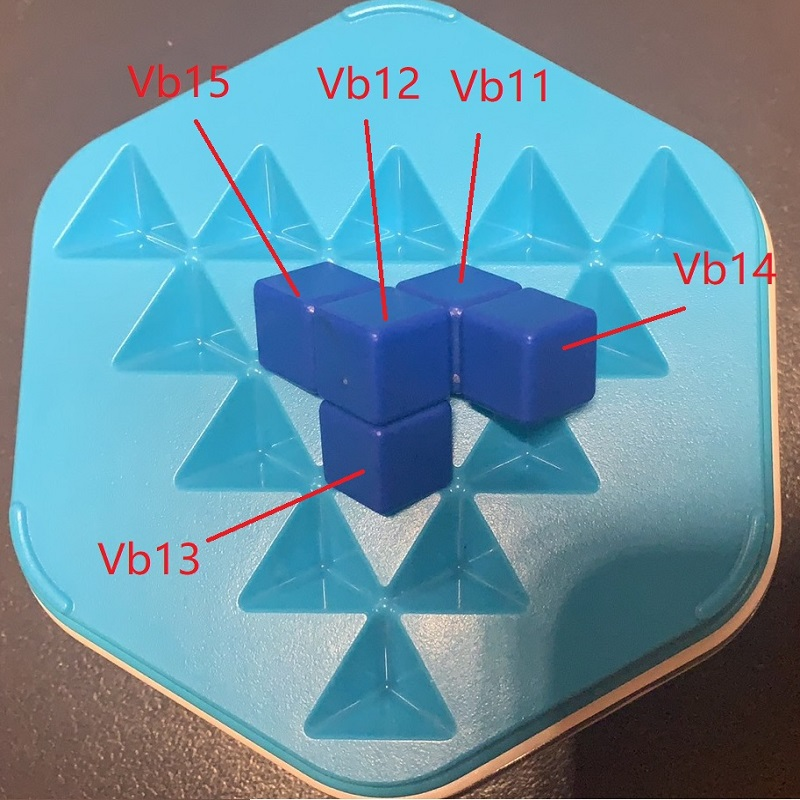
\includegraphics[width=\textwidth]{figs/3Dblue1.jpg}
\caption{The variable explanation of blue1}
  \label{fig:3Dblue1}
\end{subfigure}
\begin{subfigure}[b]{.24\textwidth}
\centering
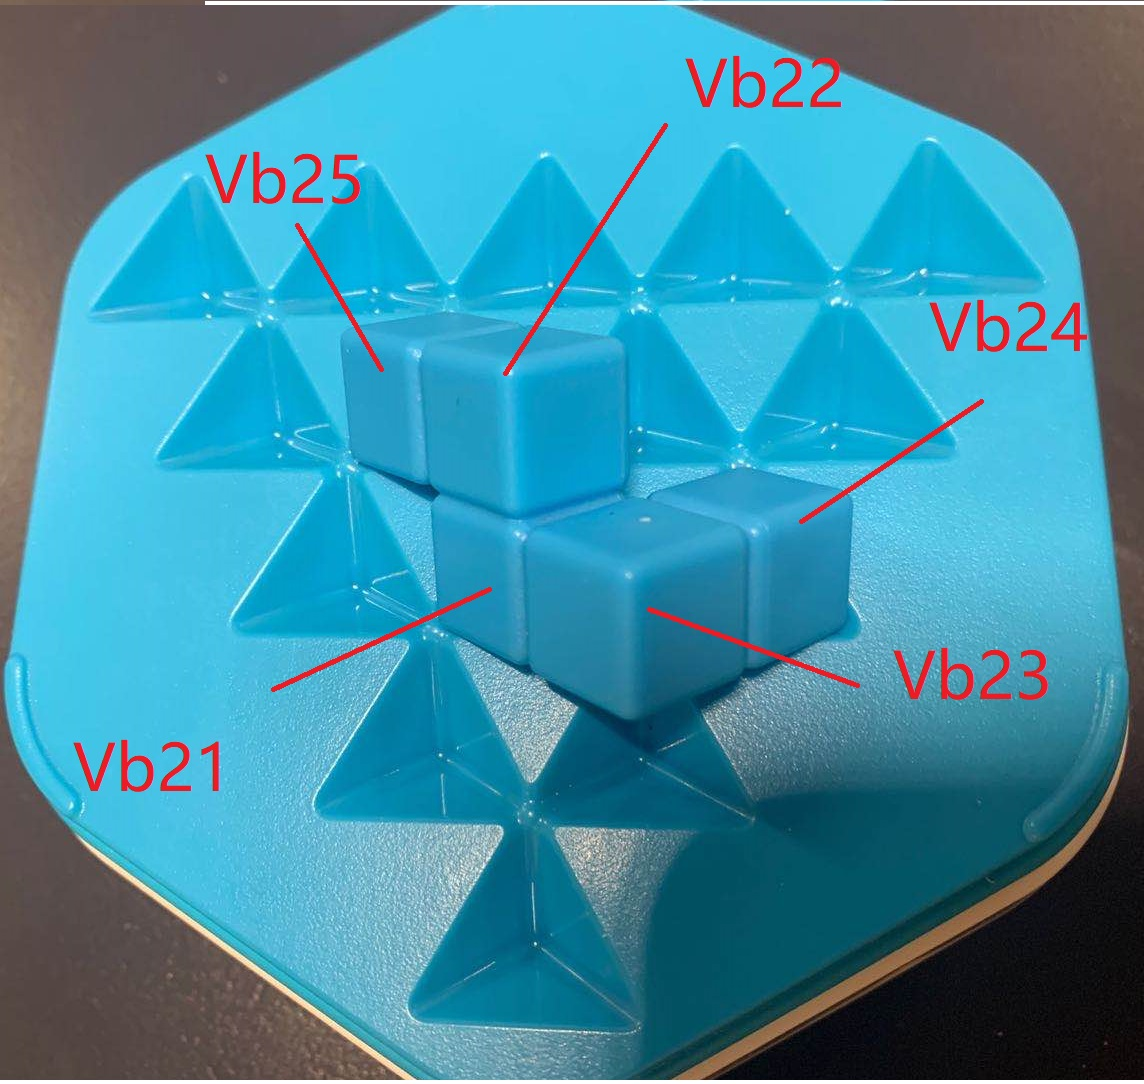
\includegraphics[width=\textwidth]{figs/3Dblue2.jpg}
\caption{The variable explanation of blue2}
  \label{fig:3Dblue2}
\end{subfigure}
\begin{subfigure}[b]{.24\textwidth}
\centering
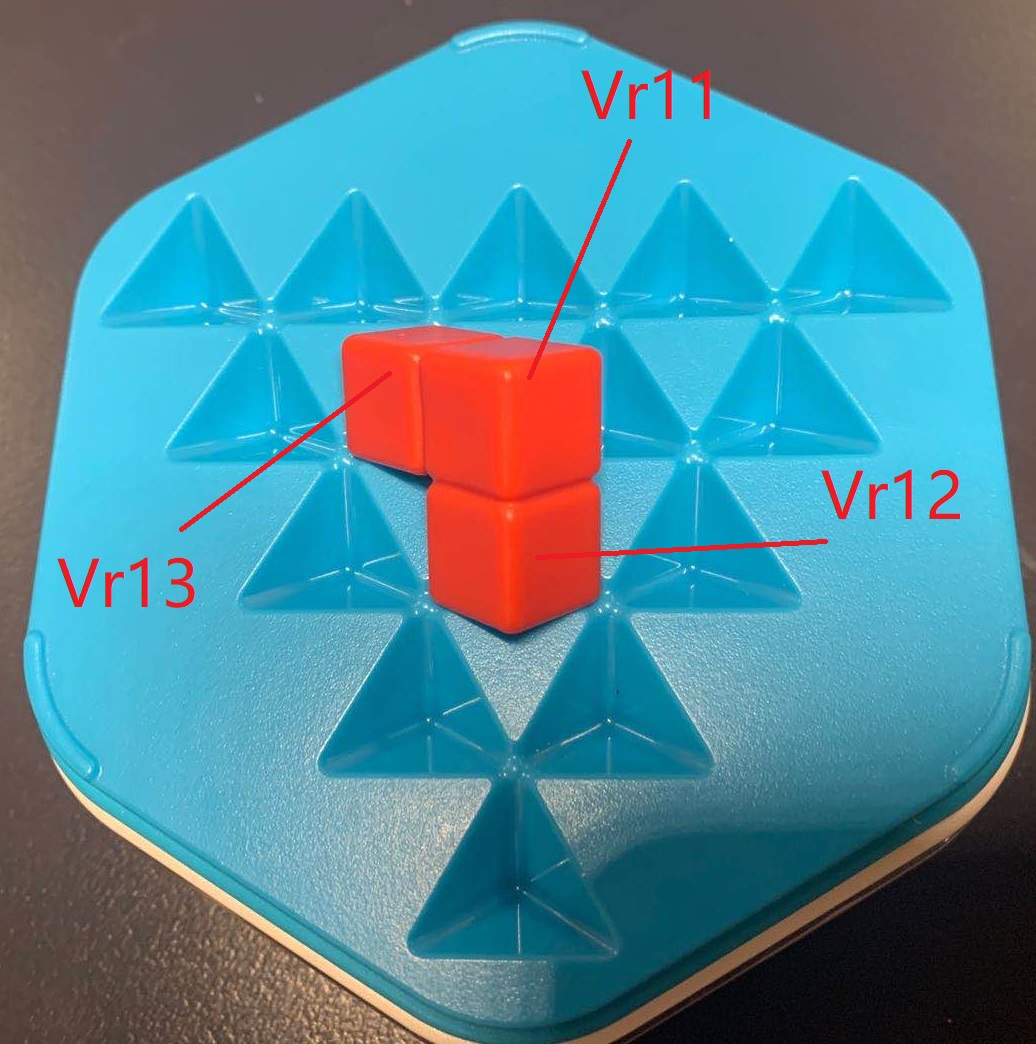
\includegraphics[width=\textwidth]{figs/3Dred1.jpg}
\caption{The variable explanation of red1}
  \label{fig:3Dred1}
\end{subfigure}
\begin{subfigure}[b]{.24\textwidth}
\centering
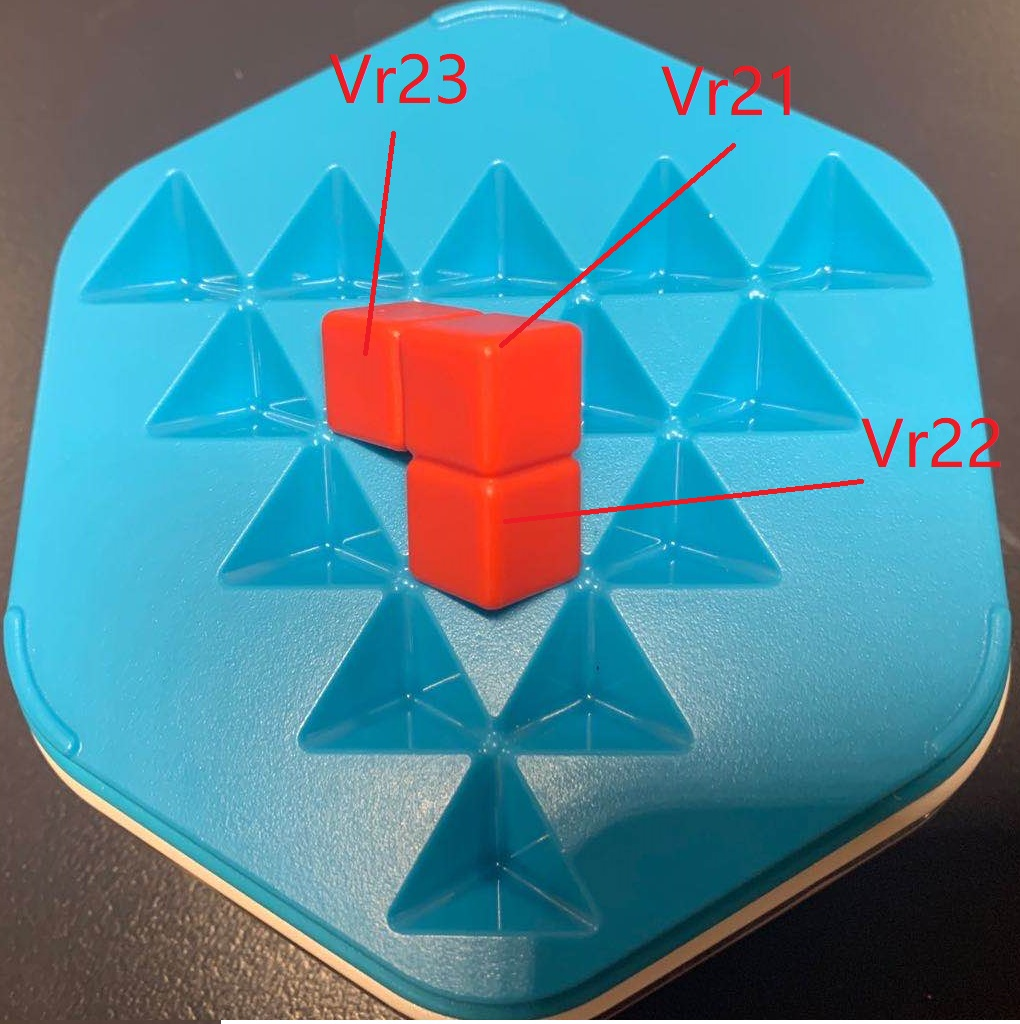
\includegraphics[width=\textwidth]{figs/3Dred2.jpg}
\caption{The variable explanation of red2}
  \label{fig:3Dred2}
\end{subfigure}
\begin{subfigure}[b]{.24\textwidth}
\centering
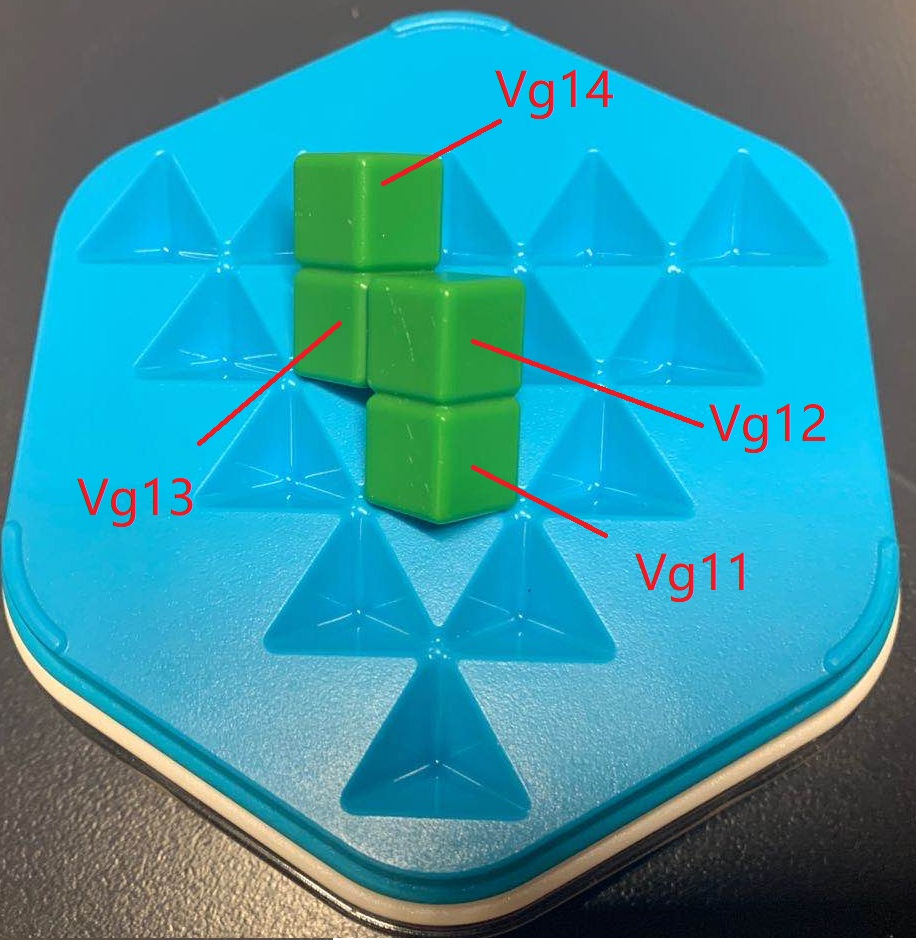
\includegraphics[width=\textwidth]{figs/3Dgreen1.jpg}
\caption{The variable explanation of green1}
  \label{fig:3Dgreen1}
\end{subfigure}
\begin{subfigure}[b]{.24\textwidth}
\centering
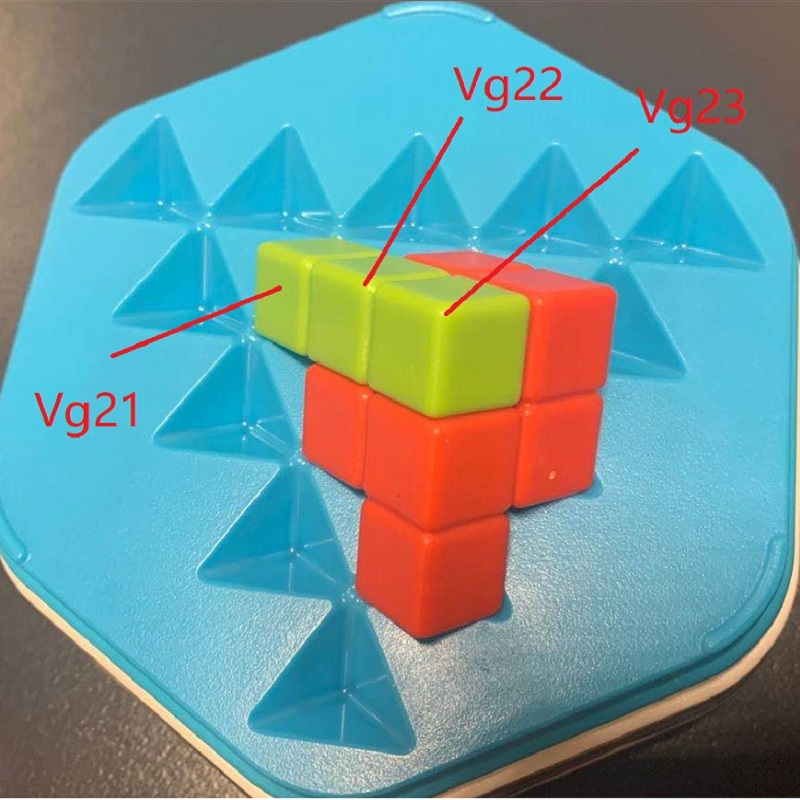
\includegraphics[width=\textwidth]{figs/3Dgreen2.jpg}
\caption{The variable explanation of green2}
  \label{fig:3Dgreen2}
\end{subfigure}
\begin{subfigure}[b]{.24\textwidth}
\centering
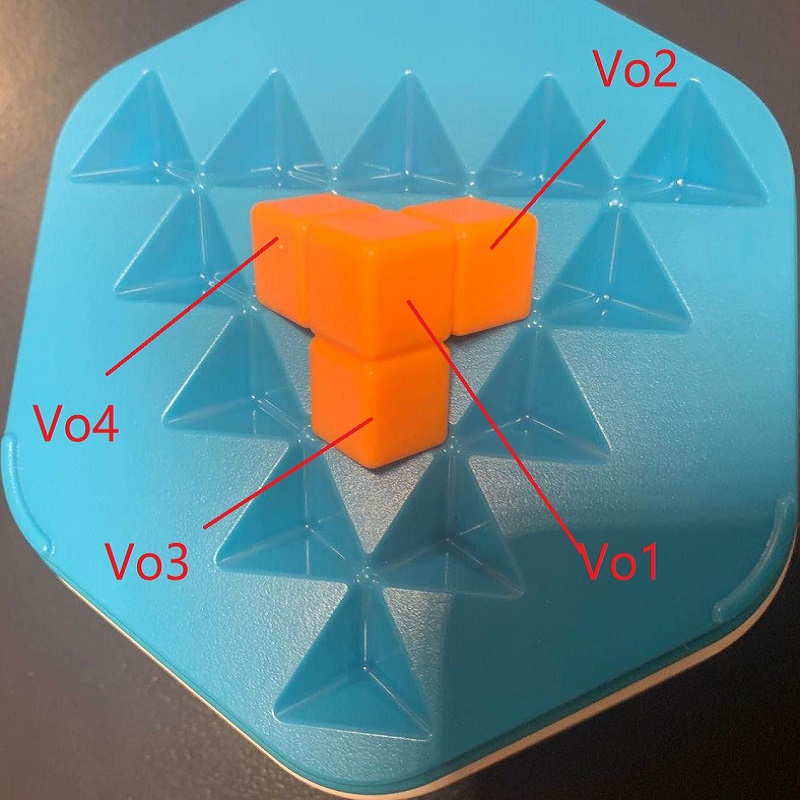
\includegraphics[width=\textwidth]{figs/3Dorange.jpg}
\caption{The variable explanation of orange}
  \label{fig:3Dorange}
\end{subfigure}
\begin{subfigure}[b]{.24\textwidth}
\centering
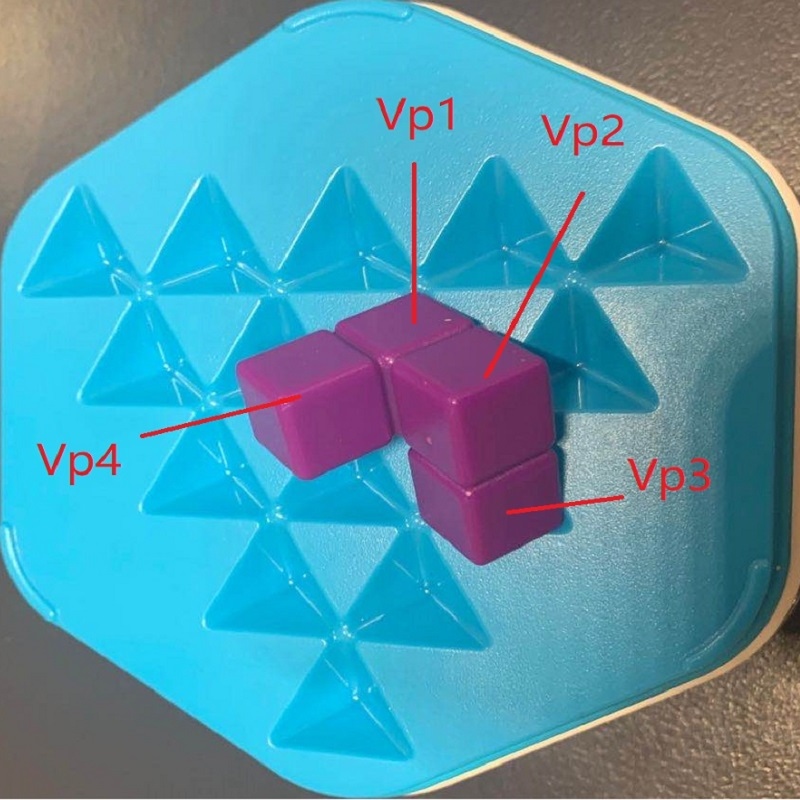
\includegraphics[width=\textwidth]{figs/3Dpurple.jpg}
\caption{The variable explanation of purple}
  \label{fig:3Dpurple}
\end{subfigure}
\begin{subfigure}[b]{\textwidth}
\centering
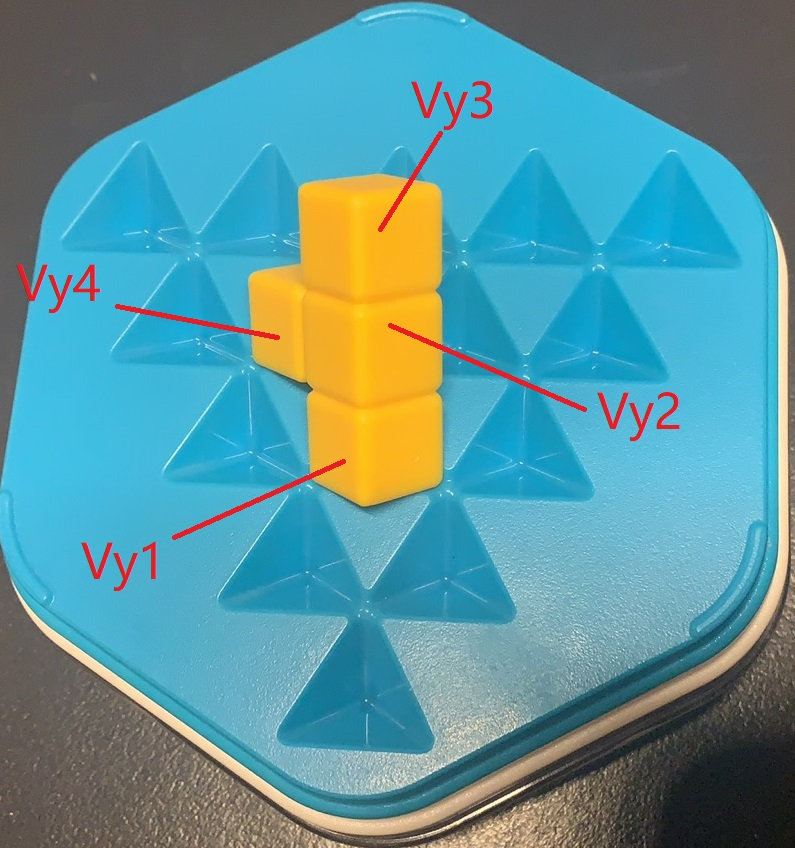
\includegraphics[width=0.24\textwidth]{figs/3Dyellow.jpg}\\
\caption{The variable explanation of yellow}
  \label{fig:3Dyellow}
\end{subfigure}
\caption{Initial state of each piece}
  \label{fig:all3Dinit}
\end{figure}
\subsection{Board for Playing Mode 1}
\label{sec:playing mode 1}
\begin{center}
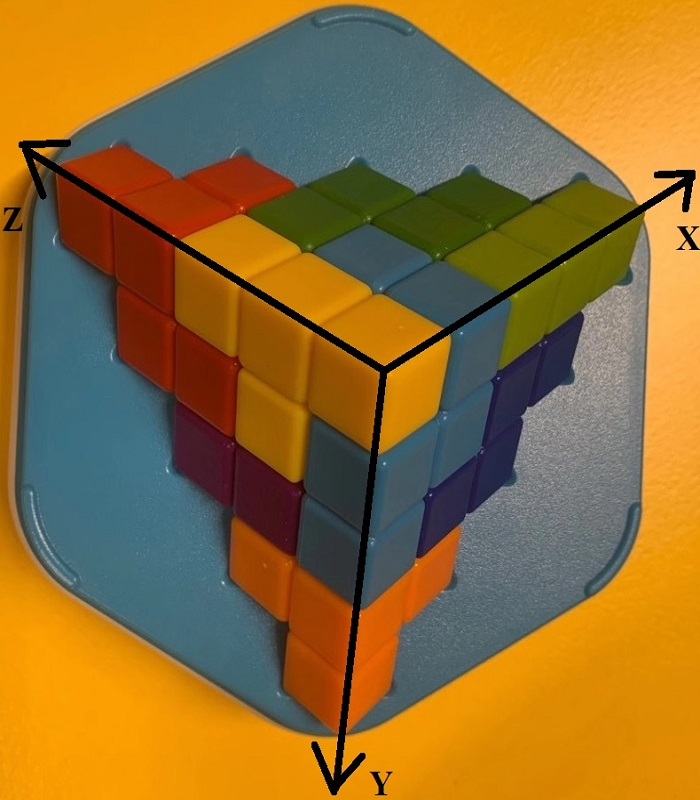
\includegraphics[scale=0.5]{figs/ZIGZAGmodel1board.jpg} \\
explanation of ZIG ZAG puzzler model1\\
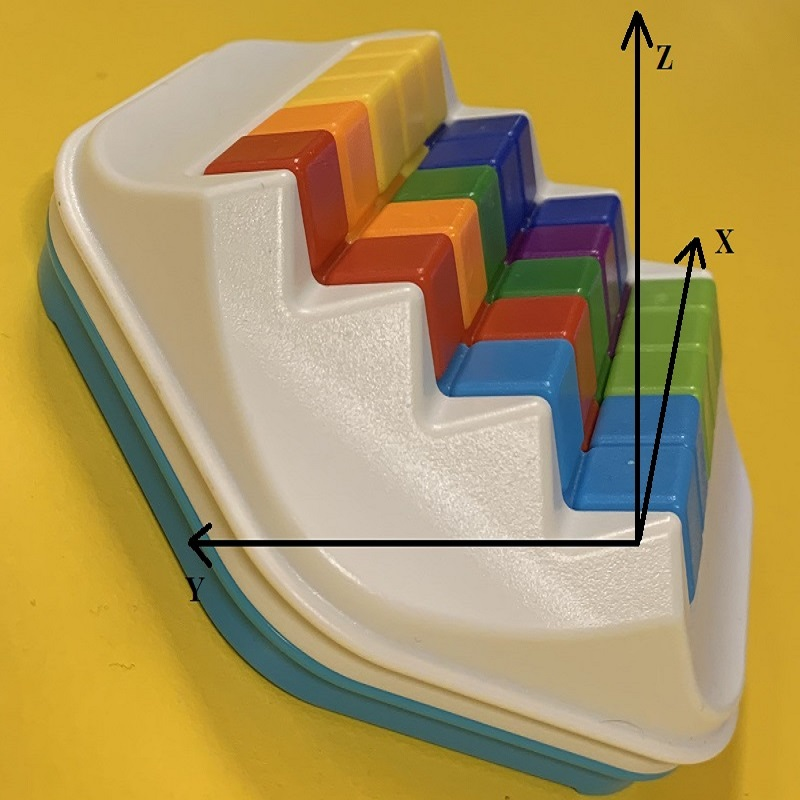
\includegraphics[scale=0.2]{figs/ZIGZAGmodel2board.jpg} \\
explanation of ZIG ZAG puzzler model2
\end{center}
\subsection{Variables for Modes 1 and 2}
\begin{align*}
\VUnits=\{&V_{y1},V_{y2},V_{y3},V_{y4},\\&V_{b11},V_{b12},V_{b13},V_{b14},
V_{b15},\\&V_{b21},V_{b22},V_{b23},V_{b24},V_{b25},\\&V_{g11},V_{g12},V_{g13},V_{g14},\\&V_{g21},V_{g22},V_{g23},\\&V_{r11},
V_{r12},V_{r13},\\&V_{r21},V_{r22},V_{r23},\\&V_{o1},V_{o2},V_{o3},V_{o4},\\&V_{p1},V_{p2},V_{p3},V_{p4}\}
\end{align*}
\subsection{Domains for Playing Mode 1}
\begin{align*}
For \hspace{1ex} all \hspace{1ex} v \in \VUnits \hspace{1ex},\hspace{1ex} D(v)=\{&(x,y,z) \in \mathbb{Z} \times \mathbb{Z}	\times \mathbb{Z} \mid  0<x \leq 5 \hspace{1ex} , \hspace{1ex} 0<y \leq 5,\hspace{1ex} 0<z \leq 5,\\& x+y\leq 6,\hspace{1ex} y+z\leq 6,\hspace{1ex}x+z\leq 6,\hspace{1ex}x+y+z\leq 7\}
\end{align*}
\subsection{Domains for Playing Mode 2}
\begin{align*}
For \hspace{1ex} all \hspace{1ex} v \in \VUnits \hspace{1ex},\hspace{1ex} D(v)=\{&(x,y,z) \in \mathbb{Z} \times \mathbb{Z}	\times \mathbb{Z} \mid  0<x \leq 5 \hspace{1ex} , \hspace{1ex} 0<y \leq 4,\hspace{1ex} 0<z \leq 4,y=z\} \hspace{1ex}\cup\\
\{&(x,y,z) \in \mathbb{Z} \times \mathbb{Z}	\times \mathbb{Z} \mid  0<x \leq 5 \hspace{1ex} , \hspace{1ex} 0<y \leq 4,\hspace{1ex} 0<z \leq 3,y=z+1\}
\end{align*}
\subsection{Constraints}
\section{Summary}
Same as the last chapter, summarize what you discussed in this chapter and
be a bridge to next chapter.
